\documentclass{report}
\usepackage[T1]{fontenc} 
\usepackage[utf8]{inputenc} 
\usepackage[backend=biber, style=ieee]{biblatex} 
\usepackage{csquotes}
\usepackage[portuguese]{babel}
\usepackage{blindtext}
\usepackage[printonlyused]{acronym}
\usepackage{hyperref}
\usepackage{graphicx}
\usepackage{color}


\begin{document}
%
% Settings
%
\def\titulo{Proj2}
\def\data{12-06-2017}
\def\autores{Mário Liberato, Jorge Oliveira}
\def\autorescontactos{(84917) mliberato@ua.pt, (84983) jorge.am.oliveira@ua.pt}
\def\departamento{DETI}
\def\curso{MIECT}
\def\logotipo{ua.pdf}
%
%CAPA %
%
\begin{titlepage}

\begin{center}
%
\vspace*{50mm}
%
{\Huge \titulo}\\ 
%
\vspace{10mm}
%
{\Large \curso}\\
%
\vspace{10mm}
%
{\LARGE \autores}\\ 
%
\vspace{30mm}
%
\begin{figure}[h]
\center
\includegraphics{\logotipo}
\end{figure}
%
\vspace{30mm}
\end{center}
%
\end{titlepage}

% Pag Titulo %
\title{%
{\Huge\textbf{\titulo}}\\
{\Large \departamento\\ \curso}
}
%
\author{%
    \autores \\
    \autorescontactos
}
%
\date{\data}
%
\maketitle

\pagenumbering{roman}

%RESUMO%
\begin{abstract}
Para o 2º projeto, o grupo tinha um objetivo: criar uma aplicação móvel onde é possível modificar imagens, aplicando um efeito, adicionar texto ou transformar em meme enviando de seguida para um servidor onde também se pode visitar uma galeria com outras imagens submetidas. Este projeto foi realizado em Python tal como alguns módulos, sendo os mais usados CherryPy e Pillow. A aplicação necessitava de ter uma \textit(frontend) onde era apresentado o conteúdo ao utilizador e uma \textit(backend) onde esta um servidor, base de dados, aplicador de efeitos e gerador de memes. A aplicação pode ser acedida de duas forma: a mais convencional é através da página web on é apletivo e de uso direto; a segunda forma é a através de um terminal de escolha do utilizador, desta forma é possível interagir de forma mais profunda com a aplicaçãom onde por exemplo poderá armazenar as imagens localmente invez de num servidor.

\end{abstract}

% Agradecimentos %
%\renewcommand{\abstractname}{Agradecimentos}
%\begin{abstract}
%\end{abstract}
%Não existem agradecimentos para este relatório

\tableofcontents
% \listoftables     
% \listoffigures    


%
\clearpage
\pagenumbering{arabic} %Numeracao fica a direita
%
\chapter{Introdução}
\label{chap.introducao} 

Neste projeto é pretendida a criação de uma aplicação móvel através da qual o utilizador possa enviar fotografias para um servidor, podendo ou não aplicar filtros. Também existe uma galeria contendo todas as imagens submetidas pelos grupos.
O documento encontra-se dividido em quatro capítulos,
sendo que no \autoref{chap.metodologia} é apresentada a metodologia seguida para a criação da página e do programa em si.
No \autoref{chap.res} são apresentados os resultados obtidos da aplicação e breve análise.
Finalmente, no \autoref{chap.conc} são apresentadas
as conclusões do projeto.


\chapter{Metodologia}
\label{chap.metodologia}

O grupo optou por utilizar Python 3 como linguagem de programação principal usufruindo do módulo Pillow e CherryPy. Para desenvolver o programa o grupo foi desenvolvendo um pouco de cada módulo até à sua finalidade.

\section{Testes}

O grupo utilizou Python3 como a linguagem de programação principal. Foram usados diversos módulos, na imagem Pillow e OpenCV, para a \textit{backend} maioritariamente CherryPy e SQLite3, e finalmente, para a \textit{frontend} o módulo Ratchet, HTML e JavaScript.
A frontend está fundida com a backend.
A aplicação e as suas funções foram testadas numa VPS Debian e num computador local a correr Windows 10, devido a problemas com o XCOA. Uma variável booleana controla o comportamento da aplicação, dizendo-lhe se está a correr no XCOA ou não.


\chapter{Descrição da aplicação}
\label{chap.desc}

\section{Página Web}

O objetivo do grupo era apresentar uma página simples e fácil de usar, usando o módulo Ratchet para compatibilidade móvel. Existiram protótipos(\ref{ProtPag}) em que devido a problemas de compatibilidade não foram implementados. Um exemplo seria a implementação de código javascript que mostrava alterações na imagem em "direto" à medida que o utilizador alterava os efeitos ou texto. 

Esta funcionalidade não foi implementada devido aos recursos utilizados no dispositivo tal como no servidor provocando grande lentidão.
\begin{figure}[b]
 \center
 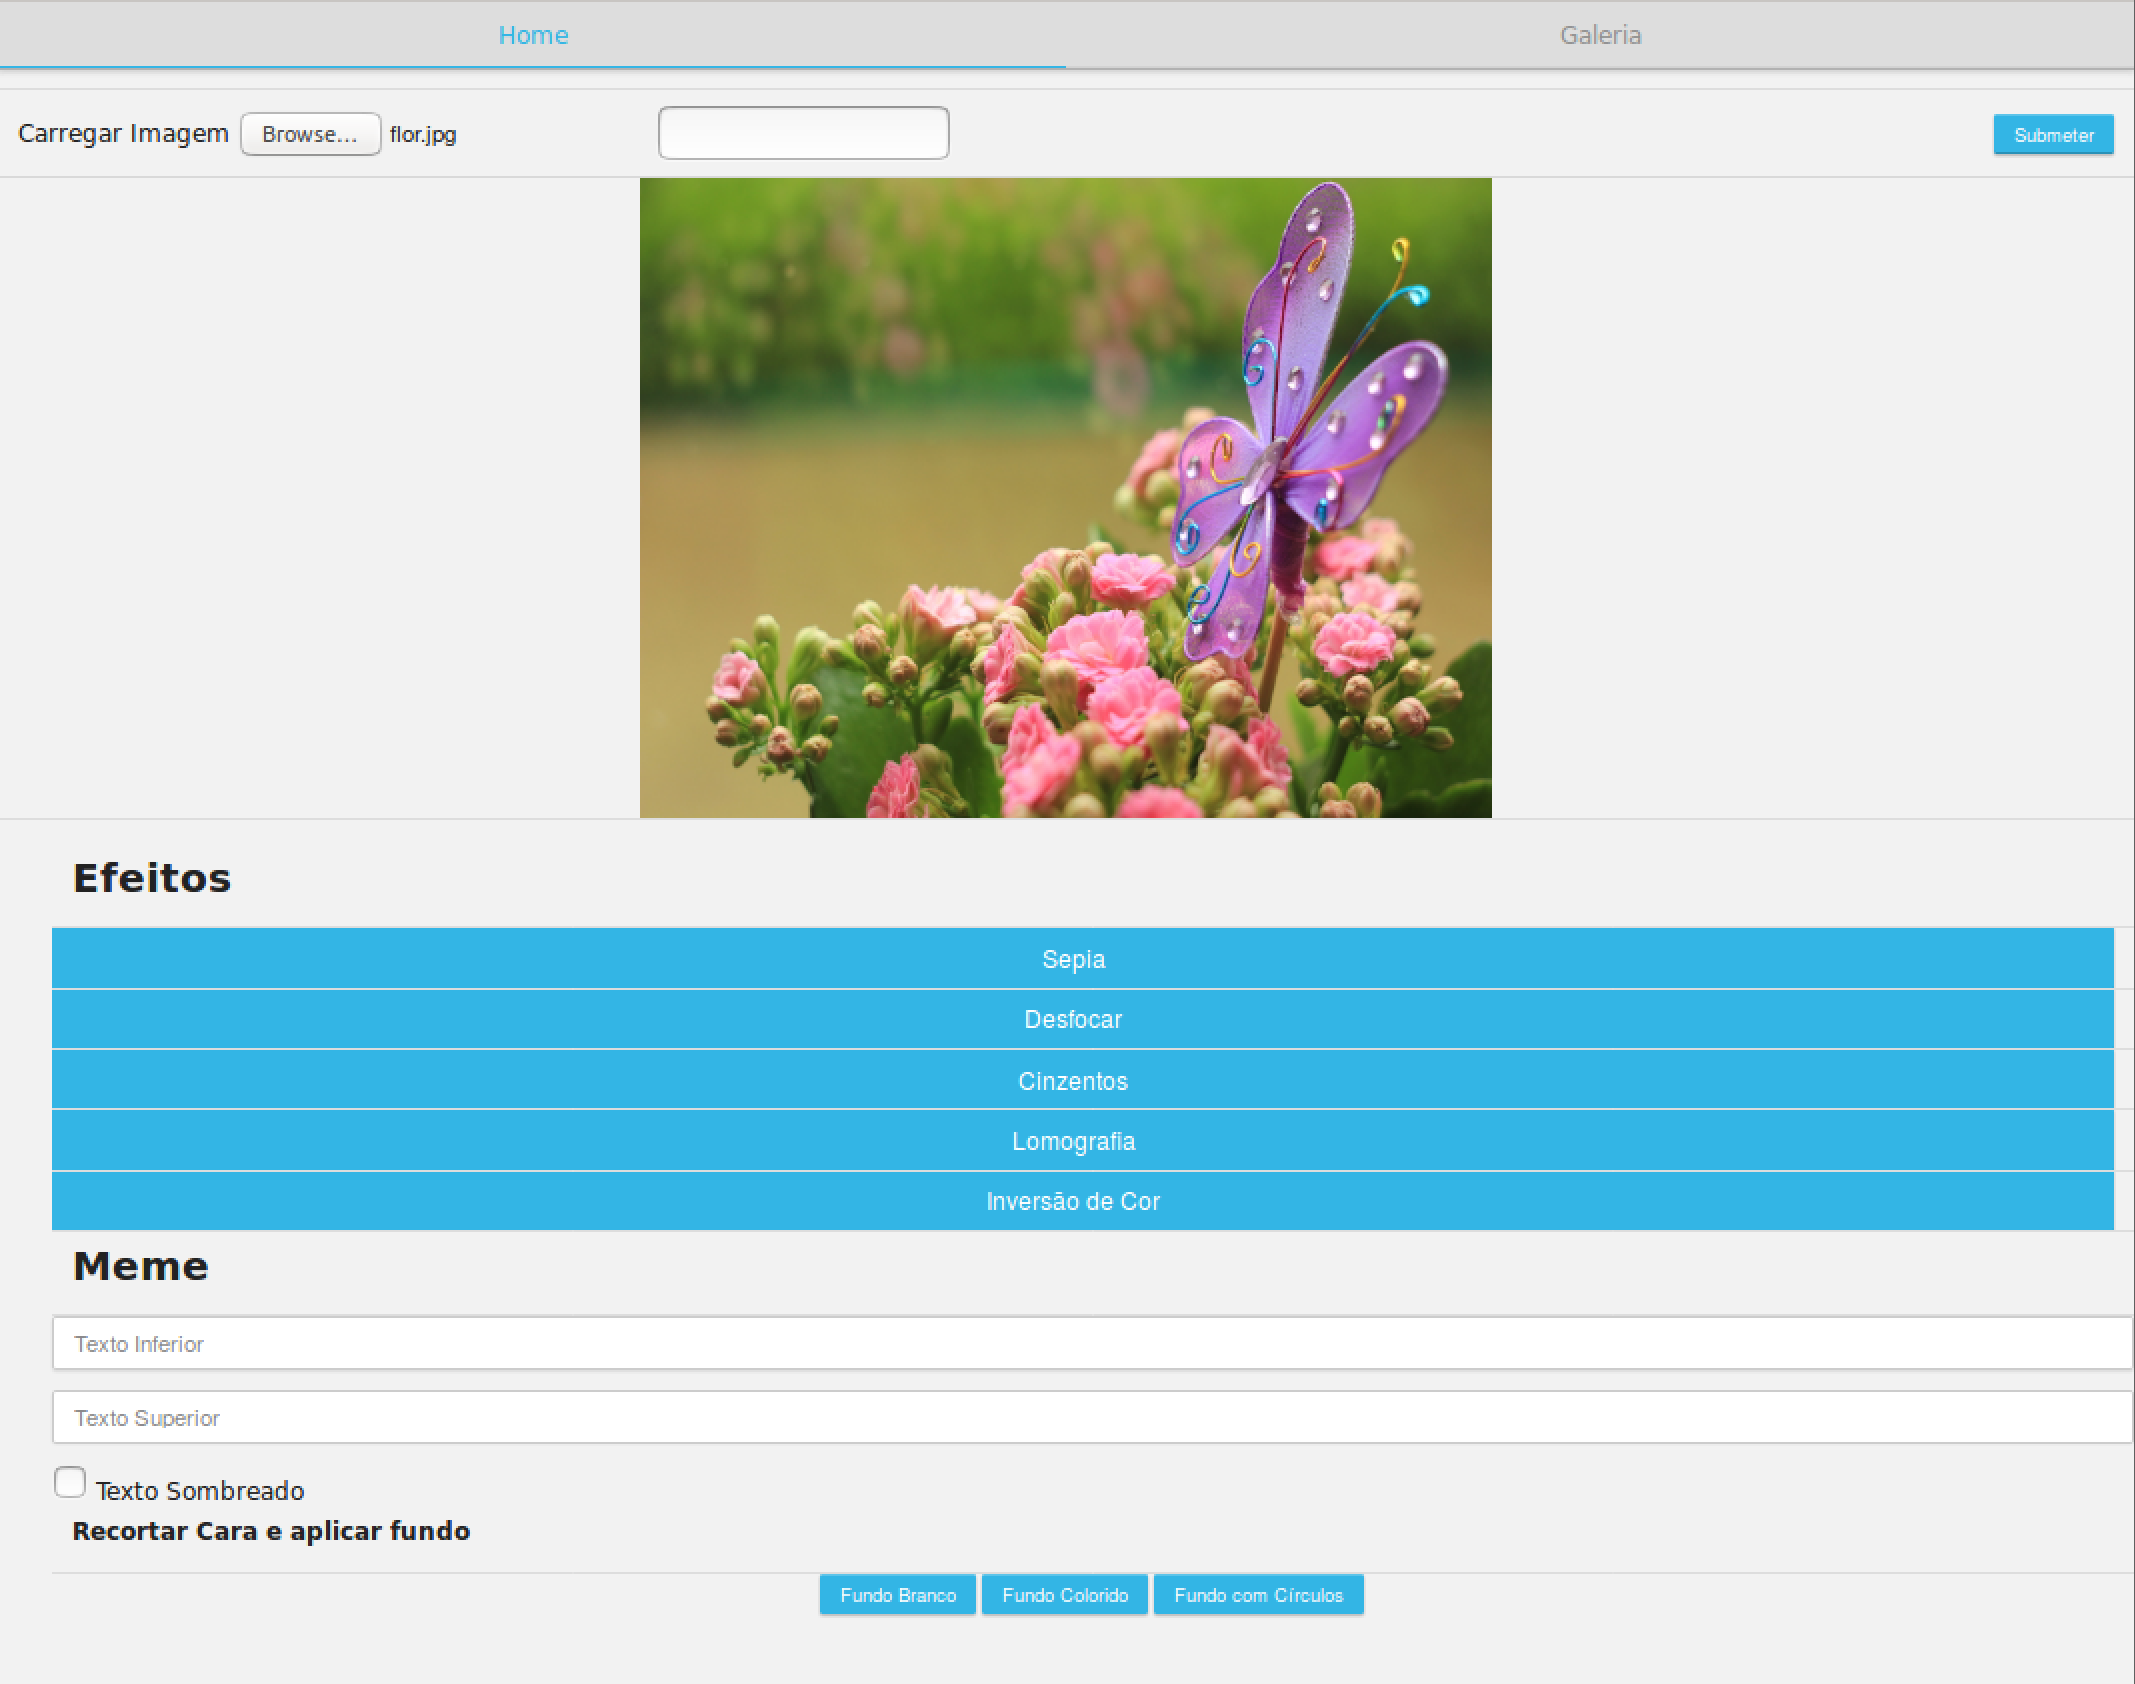
\includegraphics[scale=0.5]{prototype.png}
 \caption{Protótipo da Página(Computador)}
 \label{ProtPag}
\end{figure}



\subsection{Página Inicial}

A página inicial (\ref{HomePag}) tem carácter simples e de uso fácil. O utilizador pode selecionar uma imagem a qual é apresentada na própria página, e escolher os efeitos, ou o gerador de meme onde aplica texto e/ou um fundo à imagem. A letra da imagem ainda pode ser sombreada.
\begin{figure}[b]
 \center
 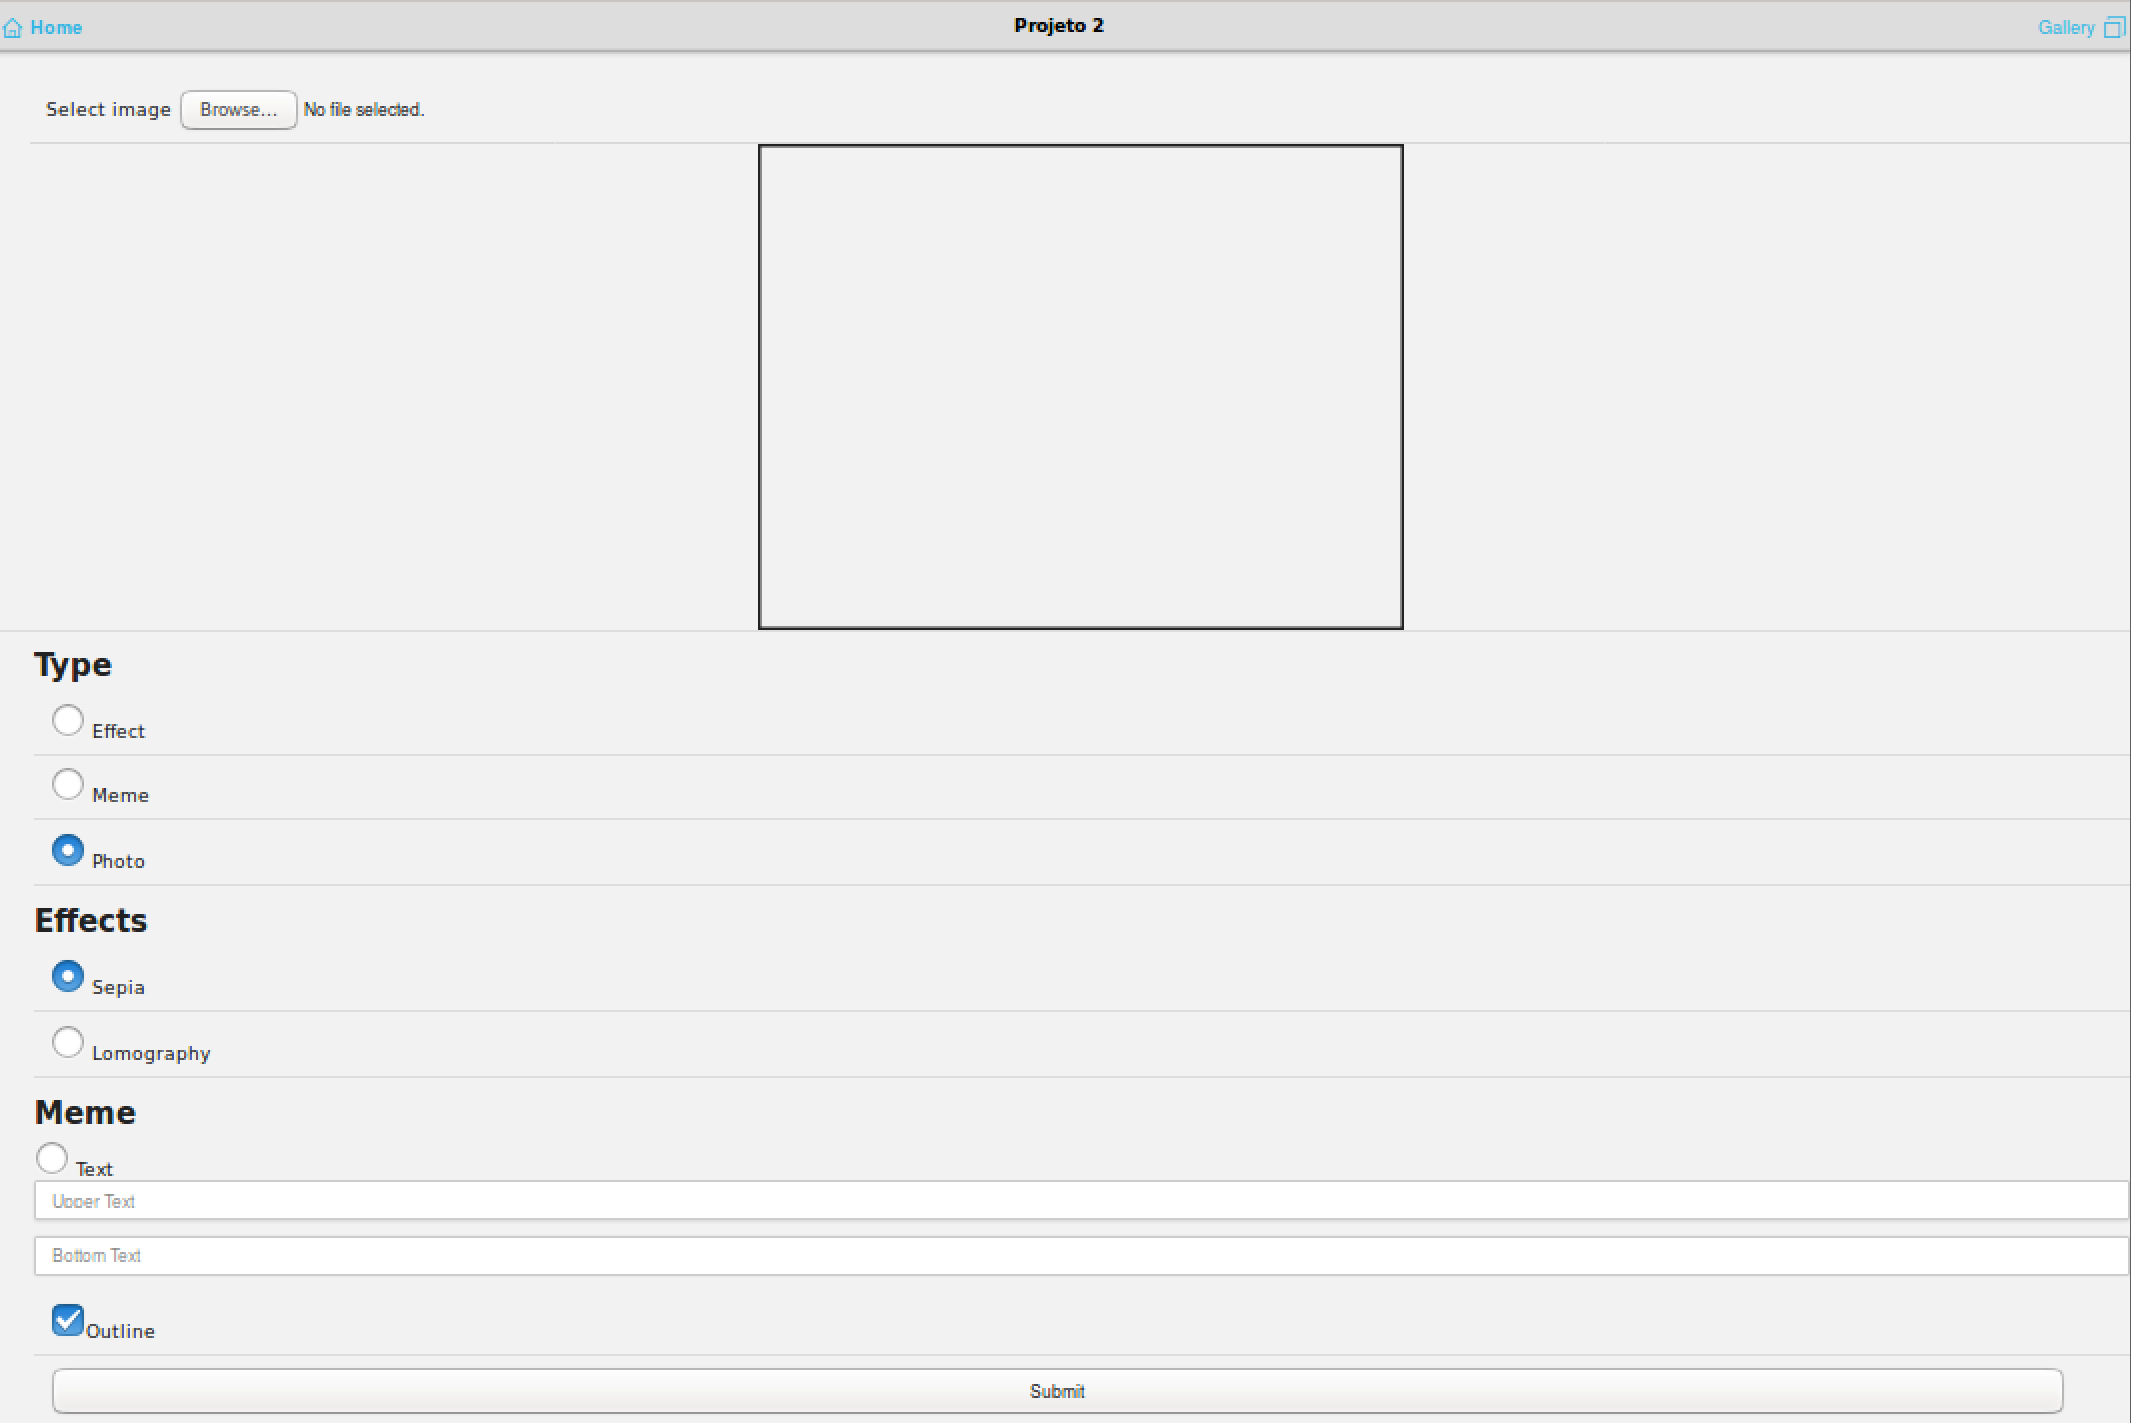
\includegraphics[scale=0.5]{final_home.png}
 \caption{Página Inicial(Computador)}
 \label{HomePag}
\end{figure}

\subsection{Submissão de Imagem}

A submissão de imagens é feita através de um método /api/put, o qual usa um pedido POST que envia a imagem e os argumentos (com os efeitos a utilizar, por exemplo). Este método faz uso de um outro método na classe API para obter um ID para a imagem a carregar antes de o fazer.

\subsection{Galeria}

A página da galeria(\ref{GalPag}) é apresentada de forma simples, também permite o utilizador realizar votos nas imagens como consultar os mesmos. A apresentação da galeria de imagens usa o método /api/listAll onde é fornecida uma lista com todas imagens dos grupos, votos e autor. Os votos são realizados através de /api/vote onde são enviados o identificador da fotografia, do utilizador e o tipo de voto.
Devido a um bug na frontend, os votos têm de ser abertos num separador novo para funcionarem.
\begin{figure}[b]
 \center
 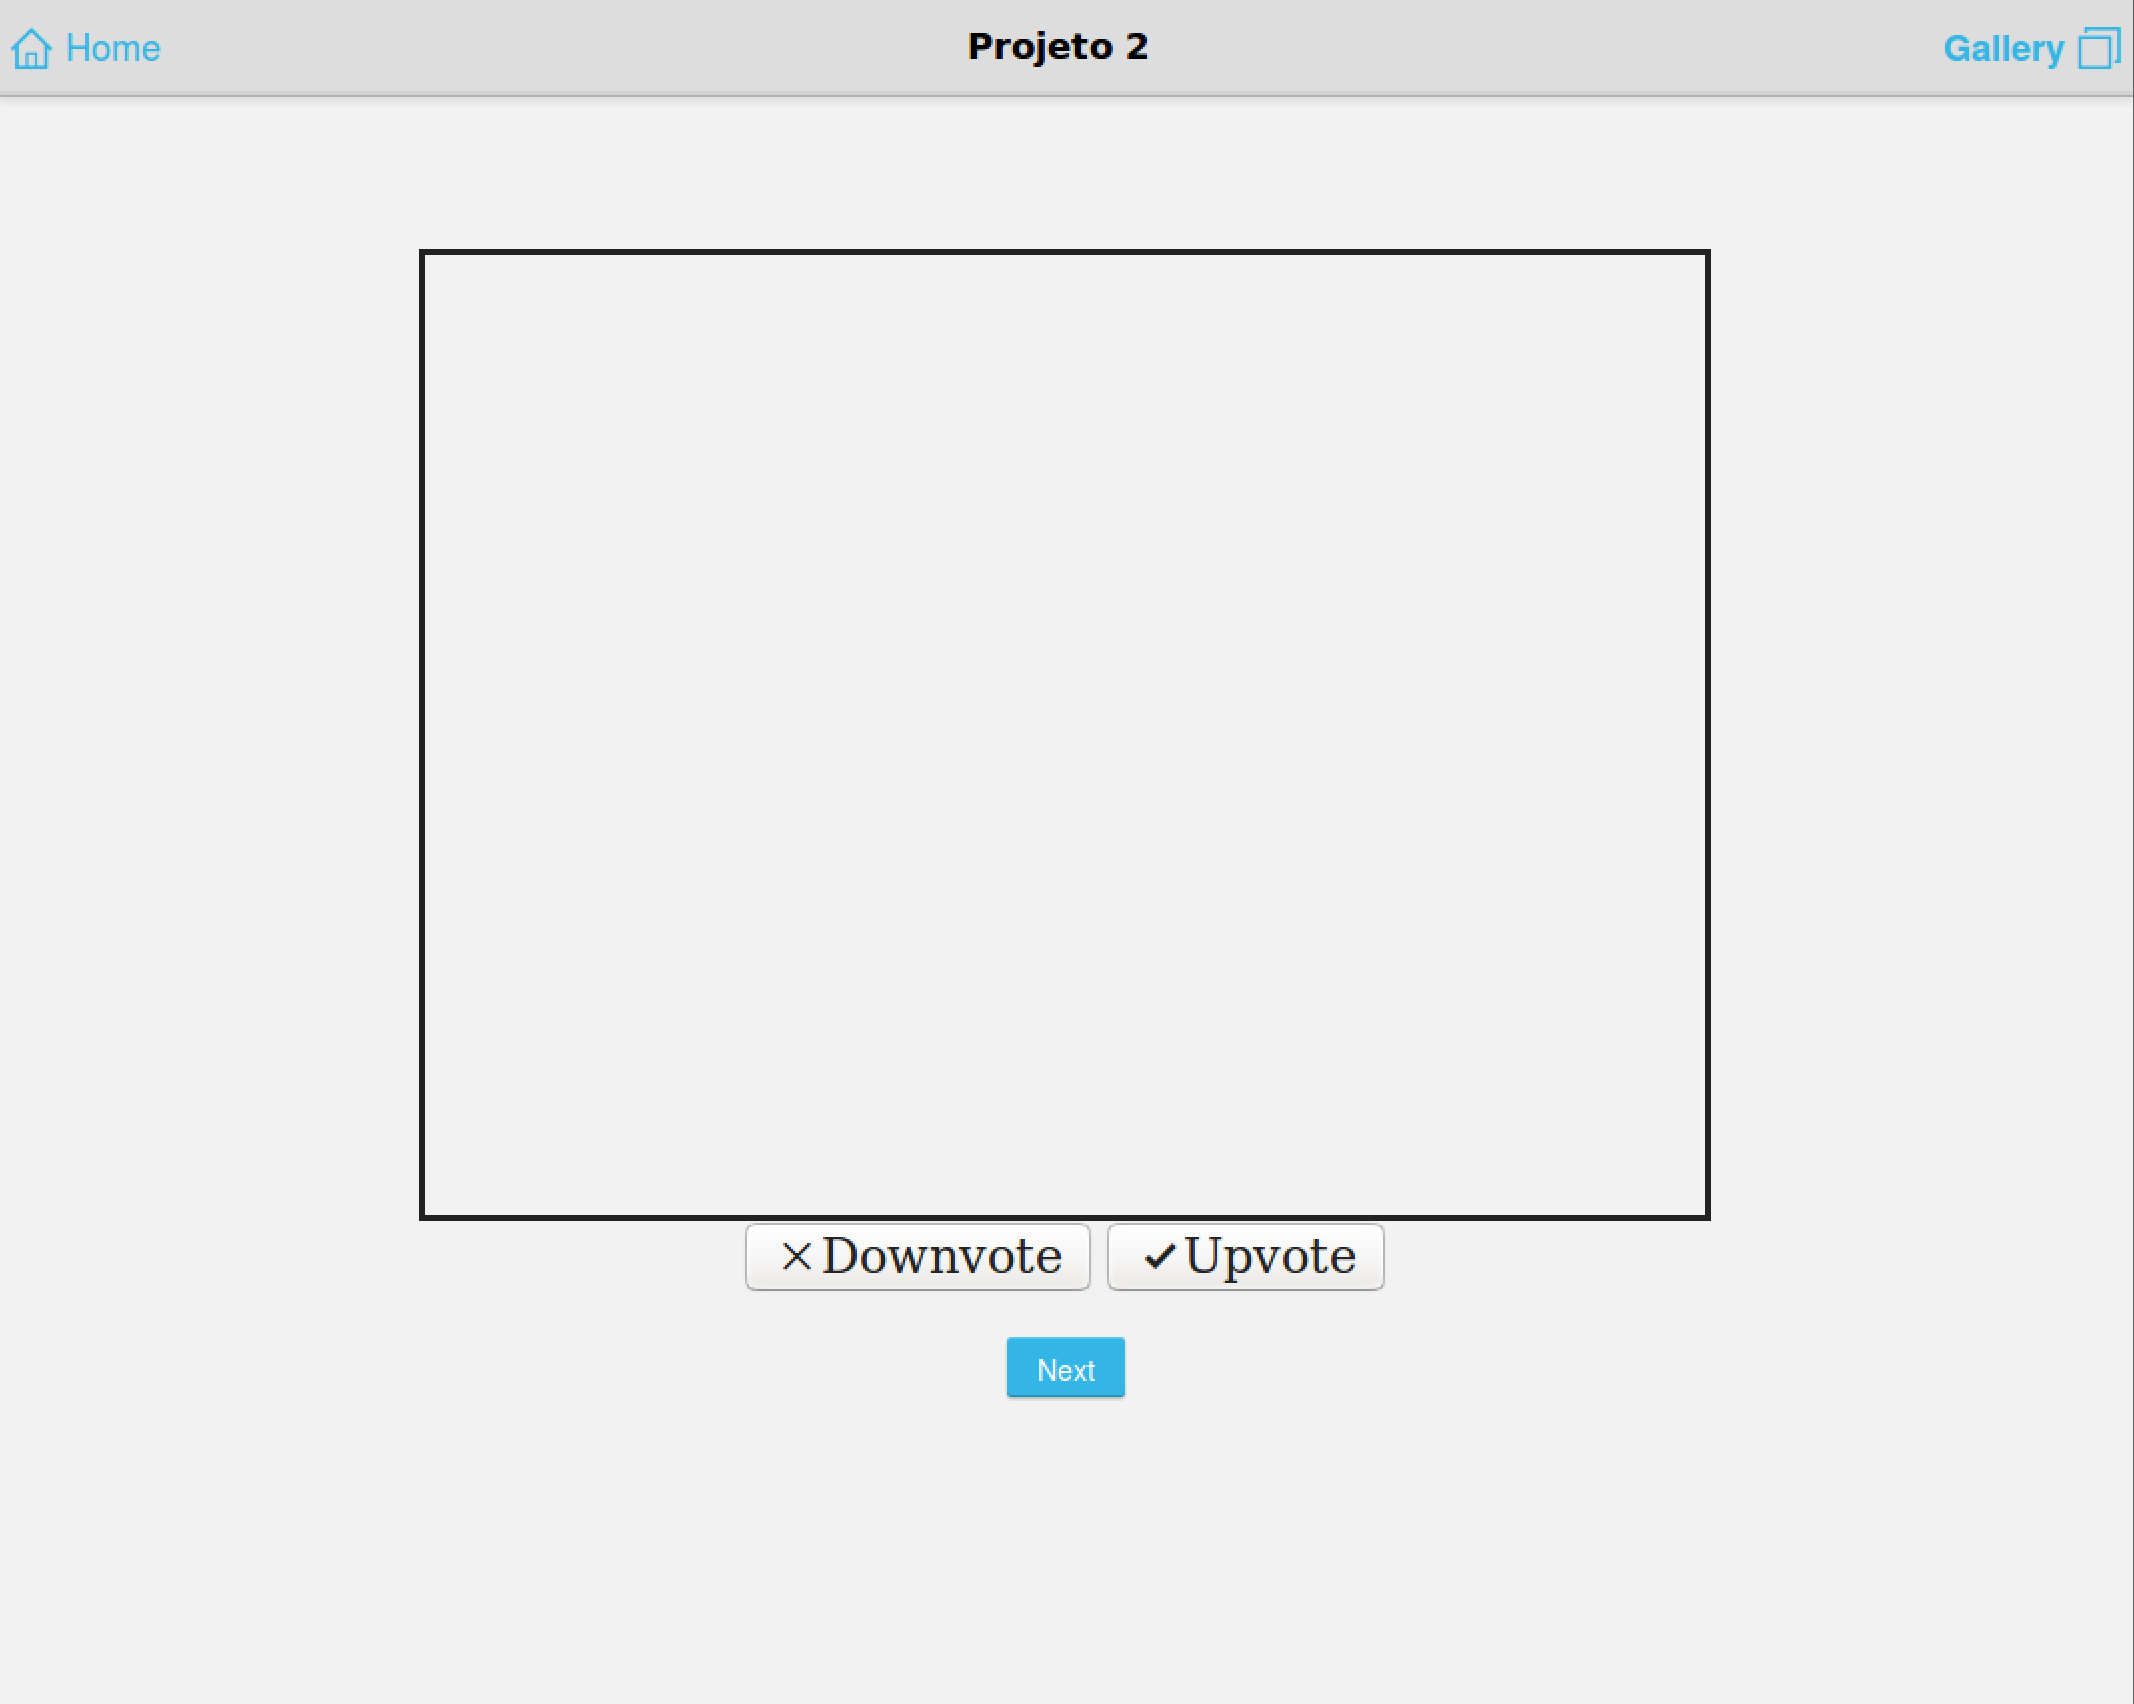
\includegraphics[scale=0.5]{final_gallery.png}
 \caption{Página da Galeria(Computador)}
 \label{GalPag}
\end{figure}

\section{Núcleo da Aplicação}

\subsection{Efeitos}

Para a realização dos efeitos foi utilizado Python3 e o módulo Pillow.
Os efeitos disponíveis no programa são: \textit{blur}, escala de cinzentos, \textit{lomography}, sépia e invesão de cor. Para a realização dos dois primeiros a imagem é processada com desfocagem e alterado o modo da imagem. Para os outros efeitos são aplicadas fórmulas matemáticas aos canais Vermelho, Verde e Azul para fazer modificações pixel a pixel à imagem.

\subsection{Gerador de Memes}

Este módulo permite aplicar texto à imagem tanto na parte inferior como superior, sombreado ou não. Também tem como objetivo recortar uma cara da imagem e por sobre um fundo colorido, à escolha do utilizador. No entanto, este módulo causou algum transtorno vistos que não foi possível existir uma forma correta de recortar uma cara de uma imagem.

\subsection{Backend}
A backend contém duas classes. Root e API. A API implementa a API pedida pelo enunciado, contendo métodos que permitem adquirir informação e interagir com a base de dados, além de fazer upload e pedido de modificação das imagens.

\chapter{Resultados e Análise}
\label{chap.res}

\section{Página Web}
	As páginas não ficaram com o aspeto inicialmente pretendido devido a problemas com JavaScript. No entanto foi possível adaptar as mesmas para ficarem fácil uso.
\section{Núcleo}	
\subsection{Tratamento de Imagem}
	O módulo dos efeito ficou feito em geral sem problemas, no entanto o mesmo não aconteceu no módulo de memes. Foram encontradas diversas dificuldades, sendo a maior delas o reconhecimento facial para recorte de uma cara, acabou por se ter de usar o módulo OpenCV para o reconhecimento dos olhos e face, sendo recortado num retângulo a cara encontrada, um problema conhecido é caso exista mais que uma cara detetada pelo algorítmo o resultado já não é o desejado. Existem dois fundos gerados pelo módulo Pillow que aplicam a cara recortada anteriormente.
	Foram criados dois ficheiros em Python distintos para aplicação de efeitos, um especial para mudança de cores e efeitos, outro para a criação dos memes. Todas as função destes ficheiros fizeram uso do módulo Pillow. Estes podem ser aplicados na própria consola do Python, importando os ficheiros e usar a função meme\_image("diretório.do.ficheiro",efeito,argumentos) 
e effect\_image("diretório.do.ficheiro",efeito).
\subsection{Backend}

\chapter{Conclusões}
\label{chap.conc}
	Apesar de não ter sido atingido o \textit{design} e funcionalidades originalmente pretendidas pelo grupo, este conseguiu criar diversas aplicações ao tratamento de imagem.


\chapter*{Contribuições dos autores}

ML trabalhou maioritariamente na backend da aplicação, realizando o servidor e a base dados tal como a adaptação dos efeitos ao servidor.

JO trabalhou maioritariamente na frontend da aplicação, dando a face ao programa nas páginas web, tal como o gerador de meme com os seus efeitos.

\chapter*{Acrónimos}
\begin{acronym}
 \acro{api}[API] {Application Programming Interface/Interface de Programação de Aplicações}
 \acro{deti}[DETI]{Departamento de Electrónica, Telecomunicações e Informática}
 \acro{miect}[MIECT]{Mestrado Integrado em Engenharia de Computadores e Telemática}
 \acro{ua}[UA]{Universidade de Aveiro}
\end{acronym}


%
%\printbibliography

\end{document}
